\documentclass[11pt]{article}
\usepackage{graphicx}
\usepackage[margin=2.5cm]{geometry}
\usepackage{array}
\usepackage{tabu} 

\title{Project Proposal: Affective Communication for Assistive Robots Using Social HRI}
\author{Katie Winkle}

\begin{document}

\maketitle

\begin{abstract}

\end{abstract}

\section{Aims and Objectives}
\subsection{Aims}
The overall aim of this project is to investigate emotional expression in robot to human communication. Specifically of interest is the potential for robot to human emotion transfer and the potential benefits this might have. This can be expressed as two key project aims:

\begin{enumerate}
\item Demonstrate whether robot to human emotion contagion can occur
\item Demonstrate the consequences of affective robot communication
\end{enumerate}

The first aim deals specifically with emotion contagion, i.e. whether a human's emotional state can be changed through interaction with an emotionally expressive robot. Regardless of the result, the second aim is to demonstrate how such emotional expression might impact on human-robot interaction (HRI); specific aspects for consideration are listed under Objective 3. Generally it is the robot's effectiveness that should be considered; however the definition of effectiveness depends on the purpose of the robot. 

\subsection{Objectives}
In order to achieve the project aims, a list of specific objectives has been derived as follows: 
\begin{enumerate}
\item Study affective communication and emotion contagion
\item Create a parameterised model for creating emotional robot expression
\begin{itemize}
\item Conduct a model evaluation experiment for refinement
\end{itemize}
\item Conduct a HRI experiment to test the effects of affective robot communication
\begin{itemize}
\item Consider human/robot task performance and human emotional state
\end{itemize}
\end{enumerate}

\section{Motivation}
The psychological phenomenon of interpersonal emotion transfer (IET) between humans is still not fully understood; however it is believed to include social appraisal and emotion contagion effects \cite{parkinson2011interpersonal}. In this context social appraisal describes a person's judgement of something being affected by the emotional response of another (i.e. affecting what they think), whereas emotion contagion describes a change in their emotional state (i.e. affecting how they feel). For example, it has been demonstrated that listening to a neutral text spoken happily or sadly can induce similar feelings in the listener \cite{neumann2000mood} and that the same household object will be rated differently if it is presented alongside a picture of a smiling or disgusted face \cite{bayliss2007affective}. In addition, there is growing evidence that emotional expression is an important and subconscious part of human communication which has evolved as a mechanism for quickly communicating a range of information such as social stature and level of threat (see \cite{tracy2015nonverbal} for a review). 

Based on this there are at least two major reasons for wanting to design a robot with IET capabilities. Firstly, if emotional expression is an important part of human communication, then a robot with such capabilities might be more lifelike, more likeable and more natural to interact with. Secondly, the effects of IET described above, e.g shaping people's judgement or decision making and impacting on how they feel might be beneficial in a range of HRI applications just as it is in human-human interaction (HHI). In fact, example HRI scenarios where emotional expression might be useful might follow directly from those we can imagine in HHI, e.g. in encouraging children or care of the unwell. As a speculative example, endowing an assisted living robot with IET  capabilities might offer the following functionality benefits: 
\begin{itemize}
\item the robot could provide more realistic and enjoyable social companionship
\item the robot could `cheer up' the user by being cheerful itself
\item the robot could give the user a positive impression of potentially undesirable tasks, e.g. taking medication or doing exercise
\item the robot could provide more effective encouragement during activities like those above
\item the robot could appear empathetic and caring, leading to a better human-robot relationship
\end{itemize}

However, this reasoning assumes that IET occurs equally well in HRI as HHI and that the effects on the human partner would be the same as if it was a human rather than a robot they were interacting with. Arguably, given the well known effect of the `uncanny valley'[REFERENCE?]; this assumption might not be valid and hence warrants further study. Research done so far suggest demonstrates that recognisable emotional expression is certainly possible in a range of robots (e.g. X X X from lit review), however the impact of this on a human's own emotional state and the robot's effectiveness is less well documented. 

In summary, the potential benefits of robot emotional expression and robot to human IET are clear. However, there is still significant uncertainty and a lack of evidence surrounding whether IET from a robot to a human can occur  and, if so, what impact this might have on the robot's effectiveness and/or the human's task performance. Addressing this uncertainty and lack of evidence in order to evaluate the real-world potential of robot-human IET forms the main motivation for undertaking this project. 

\section{Literature Review}

%What is emotional expression?
%-> what is its purpose for humans/ what impact can it have on human social interaction
%- general conclusion that bodily expression of emotion can either be done by performing a specific movement behaviour or by characterising any movement such that the emotion is recognisable from that; analogous to voice where emotion can be expressed via specific words or by how a neutral sentence is spoken. Not clear which is better but reflected in different model types eg continuous based on parameters e.g 'energetic movement' (Lim, Xu) vs discrete state e.g. the Korean work 
%-> how should we do it on a robot, so look at work already done, different models etc
%- Voice
%- Facial expression: Facial Action Coding System
%- Movement: Laban movement analysis and derived effort-shape analysis, Body Action and Posture Coding System. Want my system to gesture independent so as does not disrupt functional movement, and to avoid cross cultural issues (highlighted reference in Handbook Pg 11)
%-> Expression emotion through specific gestures also has the issue of being culture dependent rather than universally applicable; for example a 'hand purse' gesture which represents fear in France and Belgium, a query in Italy and is not used at all in North America (D. McNeill 1992 ref in Handbook). [could just leave sentence at ...rather than universally applicable].  
%- Demonstrated on robots: Lim, Xu
%
%What is emotion contagion?
%- fearful bodily expression motion produces higher activity in the emotion-related areas of the brain, happy expressions only in vision-related ones. Fearful expression also generated activity in action representation and motor areas [de Gelder 2004]
%
%What is the hypothesis for this study - i.e. are we expecting emotional expression to make a difference on task performance and if so what difference etc? Reference literature discussed above plus others. 
%
%[Psychology Background/Results]
%
%There are multiple theories concerning the social function of human emotion at the individual, dyadic, group and cultural level, based on the observed consequences they have for those groups \cite{keltner1999social}. For example... (fear contagion, information about environment etc references from keltner + others). This demonstrates the importance of emotional expression in human-human interaction and hence justifies its study in HRI. 
%
%[insight into the importance of emotional expression in human interaction and hence relevant to hri...or...demonstrates huge potential impact of emotional expression (e.g fear contagion) so basically here justify the need to understand and desire to use emotional expression in hri and maybe even more so in assisted living type] applications.
%
%It has been demonstrated that movement alone can express emotion even when static information is minimised, e.g. \cite{dittrich1996perception}, \cite{pollick2001perceiving}, Atkinson 2004 (affect folder of papers) [...] hence the way in which communication gestures are executed by the robot is likely to be important in emotion expression. lending credibility to this is the result found by XXX that the presence and pose of a robot body significantly increases emotion percievability compared to facial expression alone. ...maybe something about how this allows for emotional expression even in robots which do not have facial features etc.  
%
%Something on Laban movement analysis
%
%[Robot Applications/Work]
%
%Lim et al. demonstrated a framework for dynamically mapping the emotion in a speech sample to robot gesturing \cite{lim2011converting}. Four parameters are identified that can be measured in the speech sample and applied to the robot's gesture; these are speed, intensity, regularity and extent (SIRE). For examplesearch looking at specific gestures like arms up for surprise?]. Additionally, this is relatively simple(?) [compared to emotion generation models] because the robot requires no internal emotional state model. The framework was used to parameterise an example gesture on the NAO [more details on robot?] using actor speech samples and experiments were set up in order to test whether the resulting gesture successfully conveyed the emotional content of the original speech. The results suggest that changing the dynamics of a gesture, according to SIRE, can produce recognisable emotions at an inter-rater agreement of above 60\%. However, it was shown that in playing the original speech sample through the robot alongside the gesture had different impacts on different emotion, for example happiness was much easier to understand but anger was much harder. The authors hypothesised that this could be due to the neutral stance of the NAO, suggesting that whilst their method is designed to be independent of pose, the choice of gesture and pose is likely to be of importance in successfully conveying the desired emotion., speed is measured by the speech rate of the voice sample and applied to the velocity of the gesture. The use of SIRE means that the emotional communication is pose-independent [contrasting with other re
%
%In contrast, Xu et al. suggest that bodily emotion expression is in fact explicit and hence interrupts functional behaviour; however mood can be expressed through modification of robot behaviours \cite{xu2013mood}. Their proposed model is however similar to Lim's in that is uses parameters concerning things like speed and XXX in order to demonstrate affect. In \cite{xu2013mood} the authors host an experiment in which participants must set these parameters in order to demonstrate a desired mood when the robot is pointing or waving; therefore evaluating...  
%
%-----------------------------------------------------------------------------------------------------


Lim et al. demonstrated a framework for mapping the emotion in a speech sample to robot gesturing based on four parameters;  speed, intensity, regularity and extent (SIRE) \cite{lim2011converting}. This is based on the concept that the way a gesture is executed rather than the actual shape of the gesture can convey emotion and is more realistic for natural communication. A major benefit of this approach is that the robot requires no internal state model and can hence produce a continuous emotional spectrum which is pose-independent. The authors reported that, when implemented on a XXX NAO programmed to do a simple arm extension movement, emotion recognition based on movement alone was above 60\% and combining the parameterised movement with the original speech sample led to increased ease of understanding for happiness and sadness.   

A similar approach is taken by Xu et al. who presented a parameterised behavioural framework for changing the appearance of functional behaviours (waving and pointing) through varying general parameters such as speed and amplitude, but also more specific gesture modifications (e.g. palm up or down), in order to express a positive or negative mood \cite{xu2013mood}. This was also demonstrated on a NAO. In addition to gesture specific variation however the head, which had no pre-defined functional behaviour for the waving or pointing activities, was also utilised as an effector with two pose parameters. The author's then conducted an experiment in which participants were asked to adjust the model parameters. 

These works provided the inspiration to use a parameterised emotion generation model for this project...

\section{Risk Register}
%\begin{tabu} to \textwidth { | X[l] | X[l] | X[c] | X[c] | X[c] | }
%\begin{tabular}{|c|c|c|c|c|}
\begin{center}
	\begin{tabular}{|m{6cm}|m{5cm}|m{1.8cm}|m{1cm}|m{1cm}|}
		\hline
		Risk & Mitigation & Likelihood & Impact & \textbf{Score} \\
		\hline 
		Emotional content of designed \& implemented behaviours isn’t recognisable & Pre-test of behaviours with time to update and refine before experiment & 1 & 4 & \textbf{4} \\ 
		\hline
		Emotion generation model not ready in time for final experiment & Hand script behaviours to allow experiment to go ahead & 2 & 3 & \textbf{6} \\ 
		\hline
		Issue with hardware of robot platform preventing experiment being undertaken & Some time in plan for rescheduling, or could implement reduced experiment using virtual agent & 2 & 3 & \textbf{6} \\
		\hline 
		Cannot recruit enough participants for statistical significance in experiment & Start recruiting in sensible advance of experiment, use within rather than between subject design & 3 & 3 & \textbf{9} \\
		\hline
	\end{tabular} 
\end{center}
%\end{tabu}

\section{Timeline}
A Gantt Chart showing key project activities and their suggested time allocations is given in Figure \ref{fig:ProjectTimeline}. 

\begin{figure}
\centering
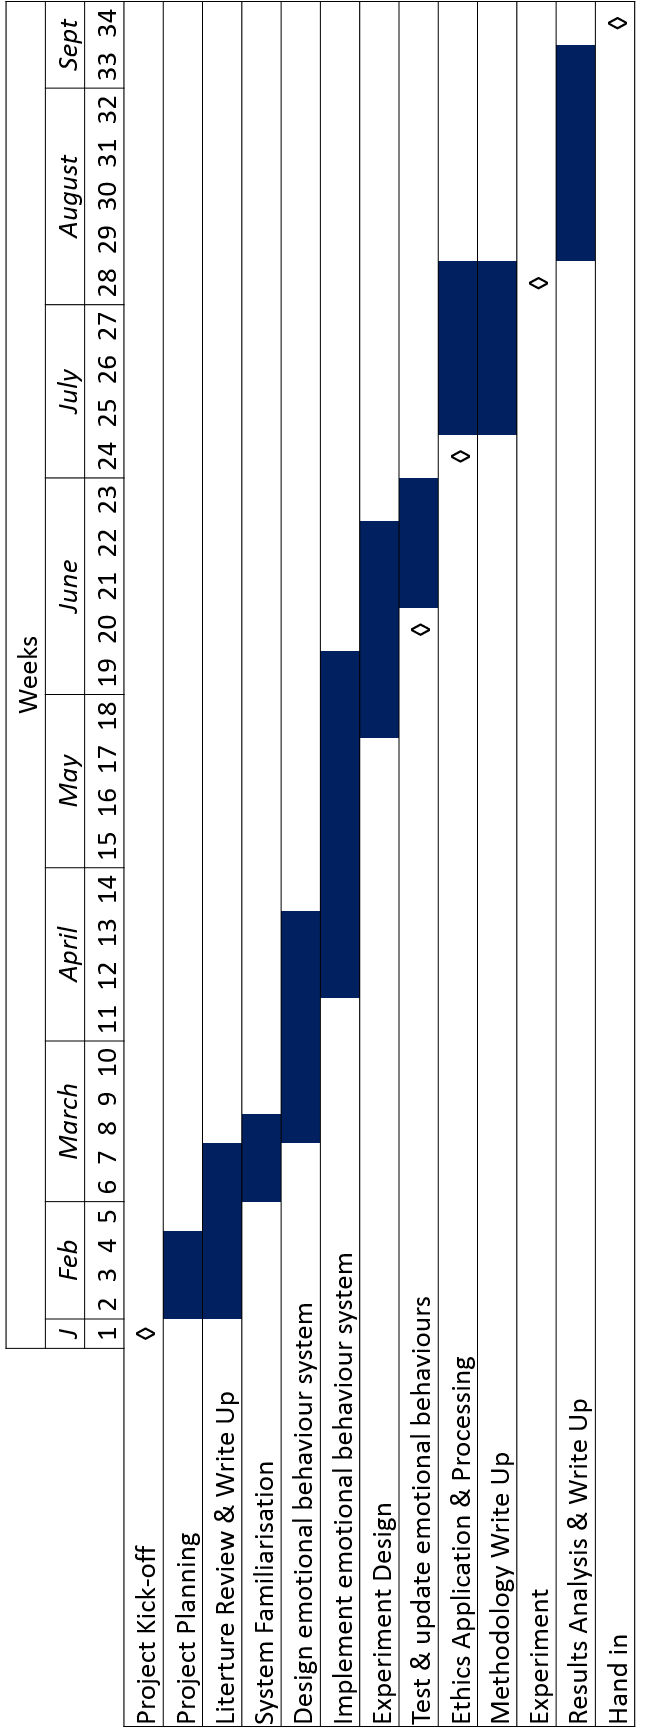
\includegraphics[height=0.9\textheight,]{ProjectTimeline2.png}
\caption{Project timeline - diamonds indicate discrete timing point events.}
\label{fig:ProjectTimeline}
\end{figure}

\bibliographystyle{unsrt}
\bibliography{ProjectReferences}
\end{document}
